\section{Experimentación Y Resultados}

\subsection{Casos de prueba}
   A continuación se listarán los casos utilizados y después se compararán los resultados.

	\begin{itemize}
		\item MOVIES: Este caso incluye 5797 páginas
		\item ABORTION: Este caso incluye 2293 páginas
		\item GENETIC: Este caso incluye 3468 páginas
		\item STANFORD: Este caso incluye 281903 páginas
	\end{itemize}   

\subsection{Comparación de Normas}

En esta sección vamos a mostrar como evoluciona la norma Manhattan (también conocida como distancia L1) entre dos vectores a medida que se suceden las iteraciones.
La norma Manhattan es la distancia entre dos vectores, o en otras palabras, la suma de la diferencia coordenada a coordenada en modulo:

\begin{figure}[h!]
   \centering
    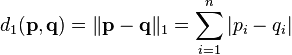
\includegraphics[width=0.5\textwidth]{imagenes/norma_manhattan.png}
\end{figure}


\subsubsection {PageRank}

Para evaluar el comportamiento de la norma manhattan variando la probabilidad del navegante aleatorio, el cual de ahora en más lo denotaremos como el parámetro \textbf{c}

Los casos de prueba se corrieron sin un limite entre normas pero si con un limite de 100 iteraciones, ya que, según lo que investigamos, con un c 	$\approx$ 0.15 la matriz suele converger en un máximo de 50 iteraciones, por lo tanto decidimos que el duplicar esto era una buena limitación. 

\begin{figure}[h!]
   \centering
    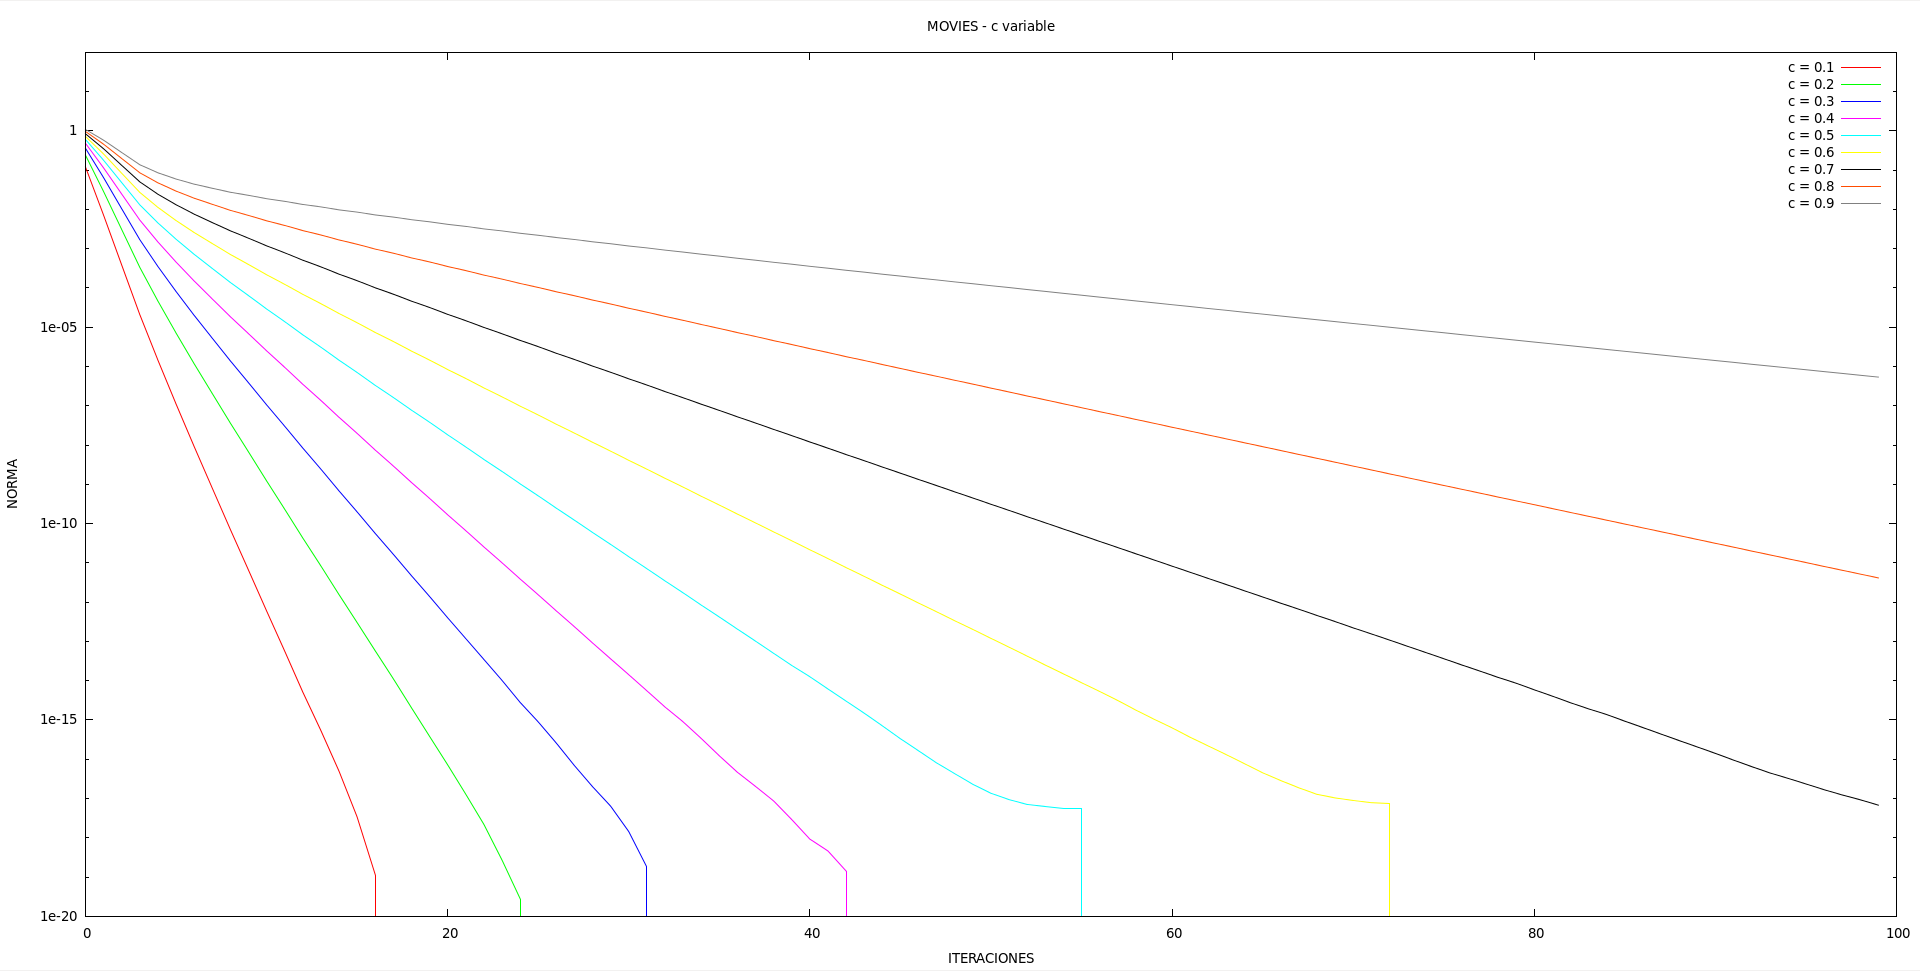
\includegraphics[width=1\textwidth]{imagenes/pagerank_norma.png}
\end{figure}

\begin{figure}[h!]
   \centering
    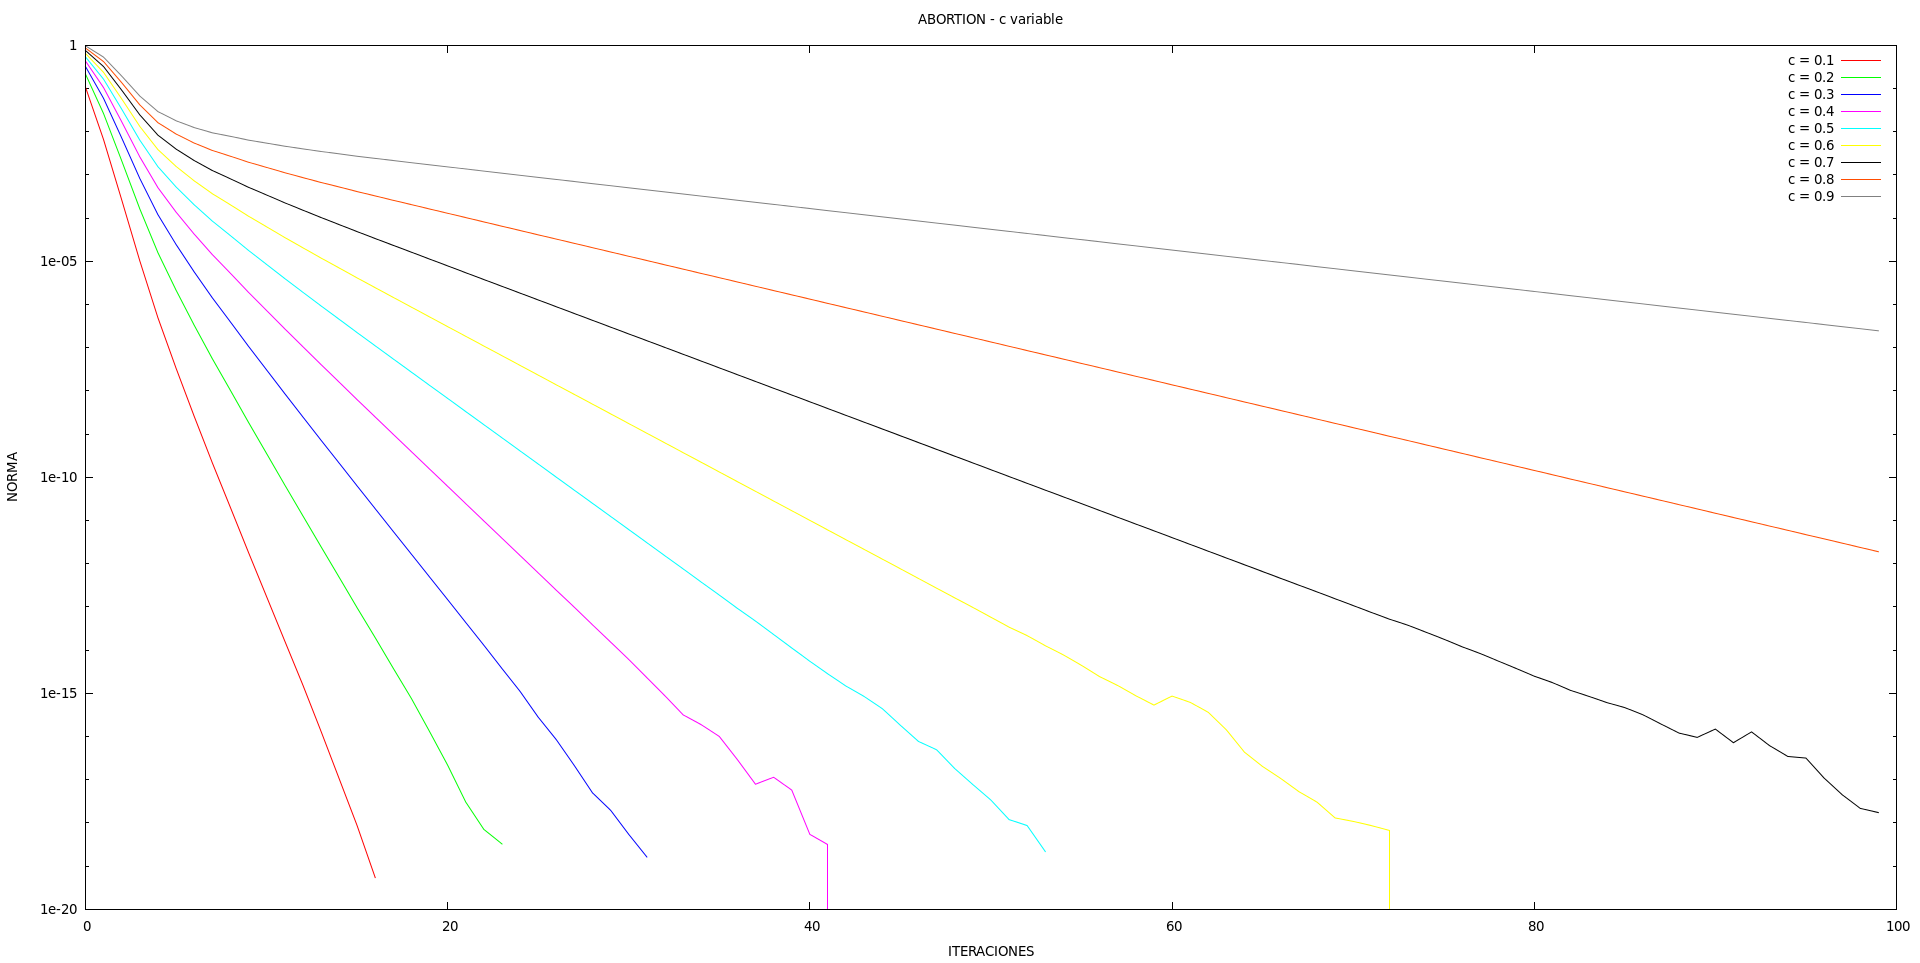
\includegraphics[width=1\textwidth]{imagenes/pagerank_abortion_norma.png}
\end{figure}

Claramente podemos notar que a medida que el C crece, el algoritmo toma más iteraciones en achicar la norma. Esto se debe a que el grado de aleatoriedad elimina el peso de la unión entre los sitios e indica una uniformidad en el comportamiento, entonces la matriz si bien estocástica ahora se encuentra distribuida esa suma $=$ 1 por columna en varias filas. Esto produce mayor cantidad de iteraciones en el método de la potencia ya que la mayor uniformidad de la matriz provoca que ninguna 'zona' de la matriz absorba más que las demás.   $[1]$
\newpage

\subsubsection {HITS}
\subsection{Comparación de Tiempos}
 
